\subsection{Verifica dei processi}

\subsubsection{Estimated at Completion}
\begin{figure}[h]
	\centering
	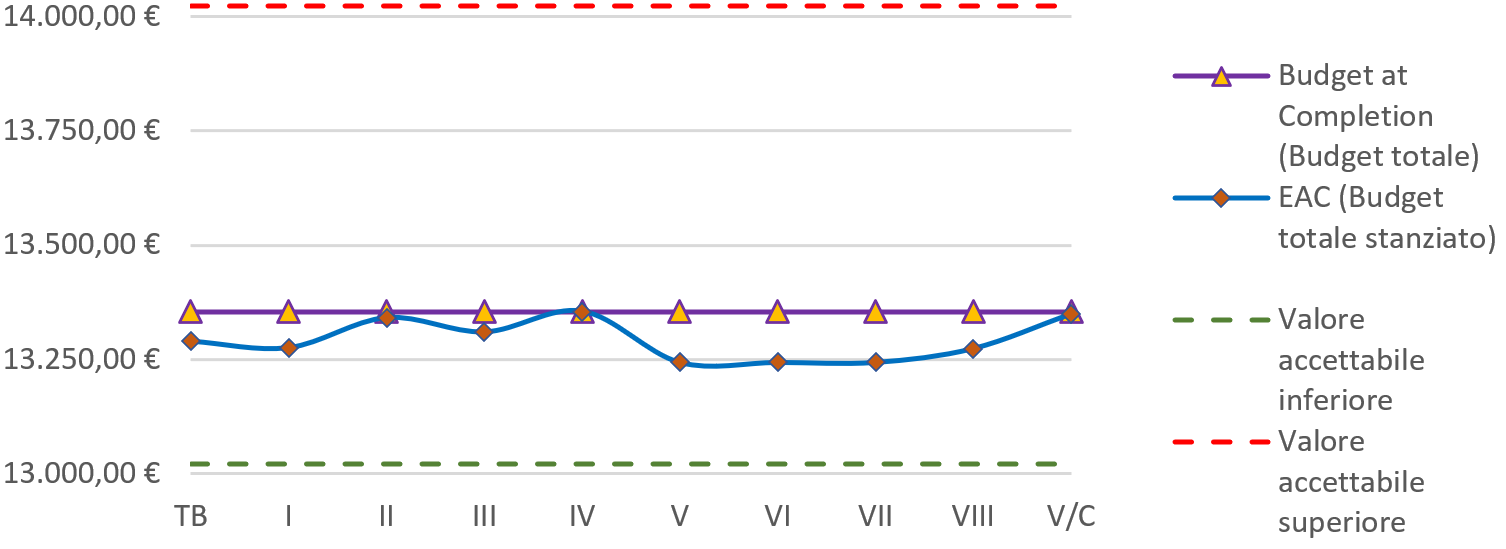
\includegraphics[width=17cm]{Images/BAC-EAC}
	\caption{Revisione del valore stimato per la realizzazione del progetto.}
\end{figure}

\newpage

\subsubsection{Actual Cost e Estimate to Complete}
\begin{figure}[h]
	\centering
	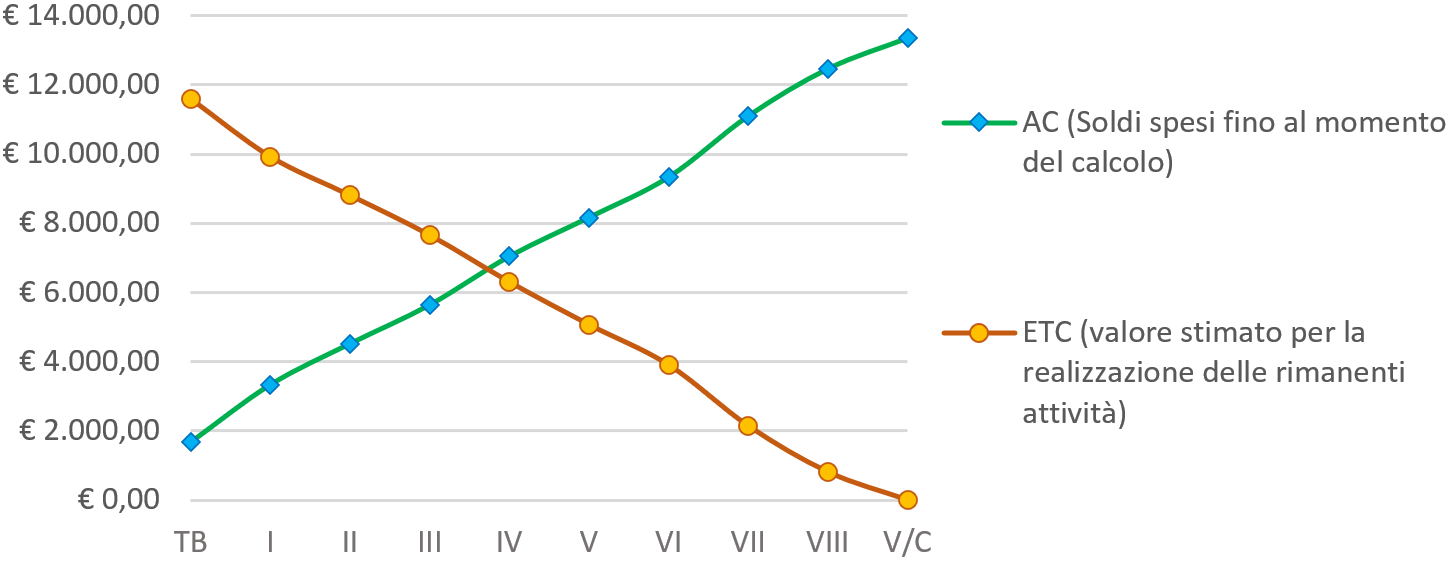
\includegraphics[width=17cm]{Images/ETC-AC}
	\caption{Costo effettivamente sostenuto e valore stimato per la realizzazione delle rimanenti attività.}
\end{figure}


\subsubsection{Earned Value e Planned Value}
\begin{figure}[h]
	\centering
	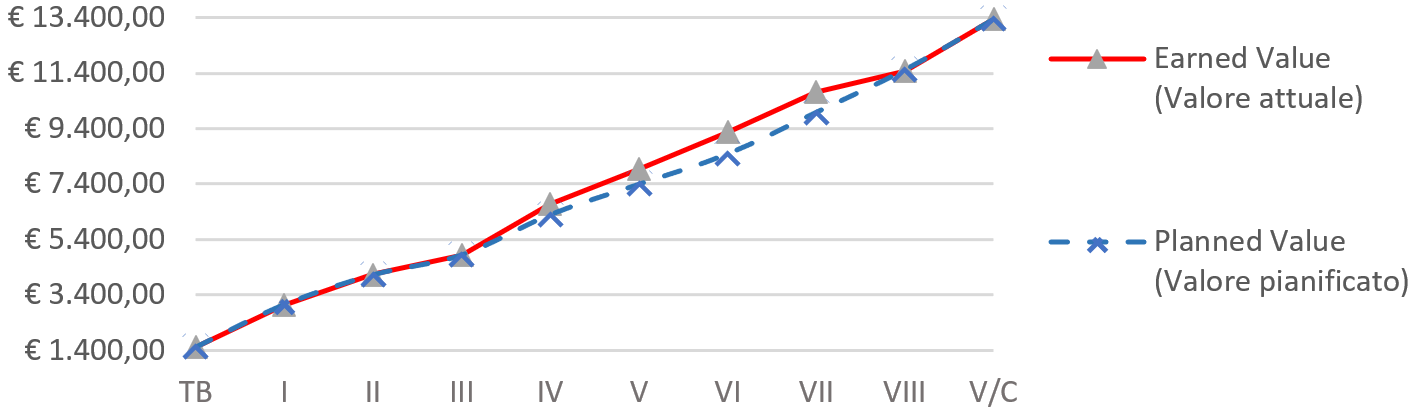
\includegraphics[width=17cm]{Images/EV-PV}
	\caption{Valore delle attività realizzate e costo pianificato per realizzare le rimanenti.}
\end{figure}

\newpage

\subsubsection{Schedule Variance e Budget Variance}
\begin{figure}[h]
	\centering
	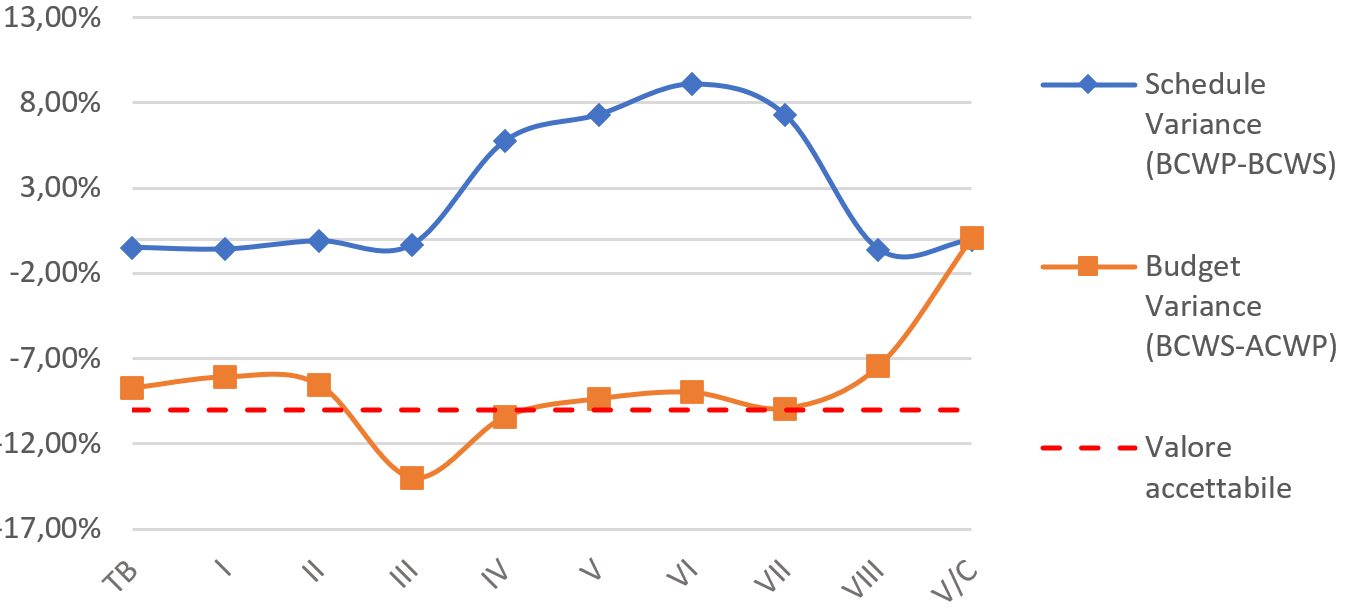
\includegraphics[width=16cm]{Images/SV-BV}
	\caption{Schedule Variance e Budget Variance per incremento.}
\end{figure}



\subsubsection{Requirements Stability Index e Satisfied Obligatory Requirements}
\begin{figure}[h]
	\centering
	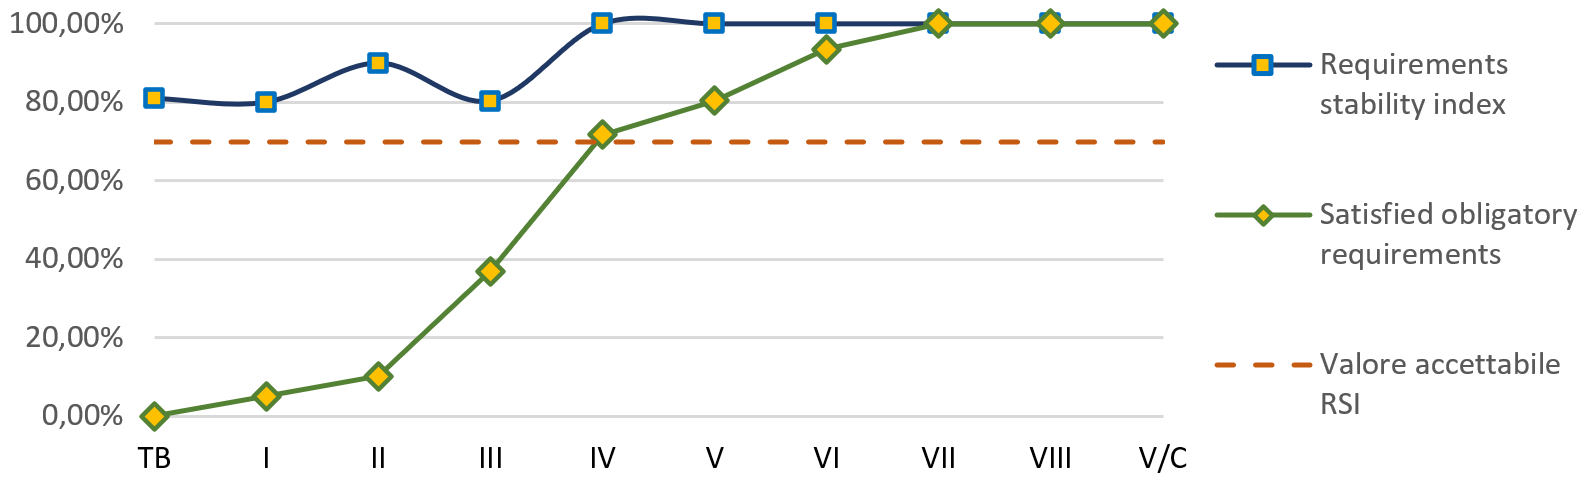
\includegraphics[width=16cm]{Images/requisiti}
	\caption{Variazione del numero di requisiti e completamento di quelli obbligatori.}
\end{figure}

\newpage

\subsubsection{Attualizzazione rischi}
\begin{figure}[h]
	\centering
	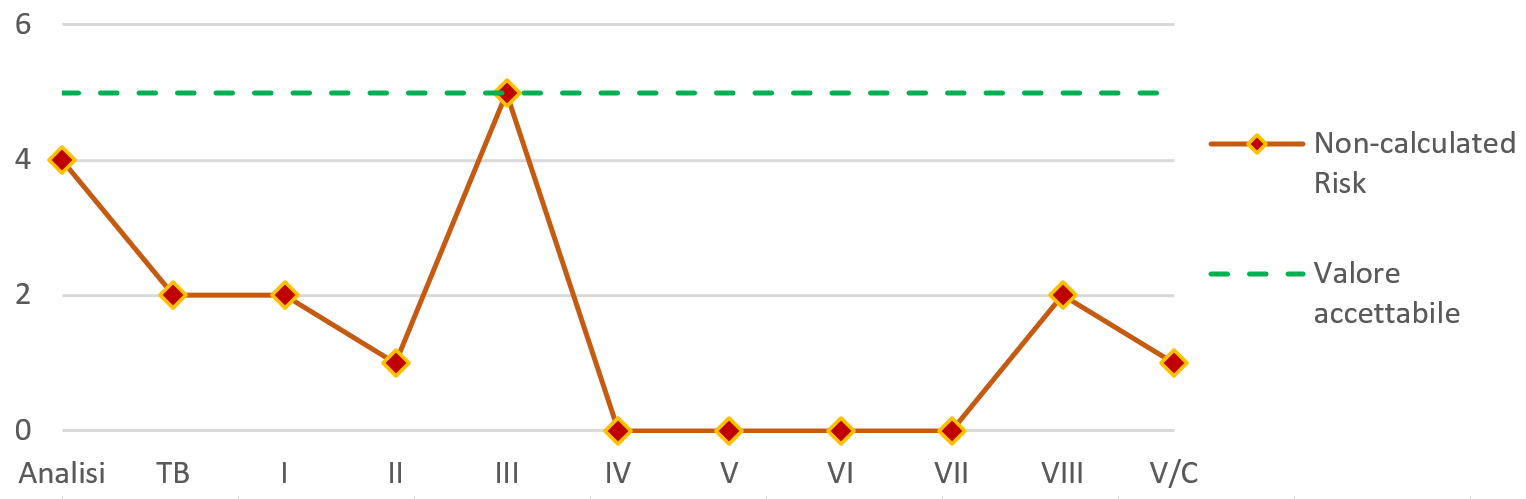
\includegraphics[width=17cm]{Images/rischi}
	\caption{Rischi preventivati verificati per incremento.}
\end{figure}



\subsubsection{Quality Metrics Satisfied}
\begin{figure}[h]
	\centering
	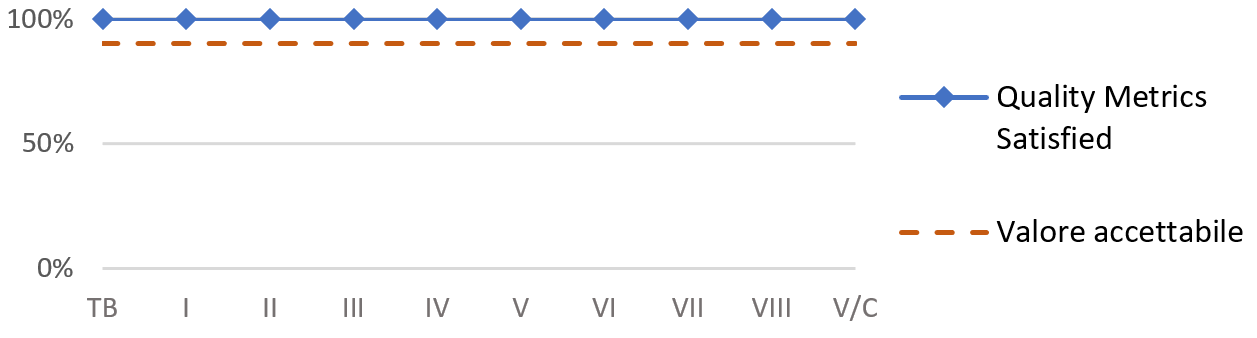
\includegraphics[width=16cm]{Images/metriche}
	\caption{Percentuale metriche di qualità soddisfatte.}
\end{figure}

\newpage

\subsubsection{Code coverage e percentuale di test superati/falliti}
\begin{figure}[h]
	\centering
	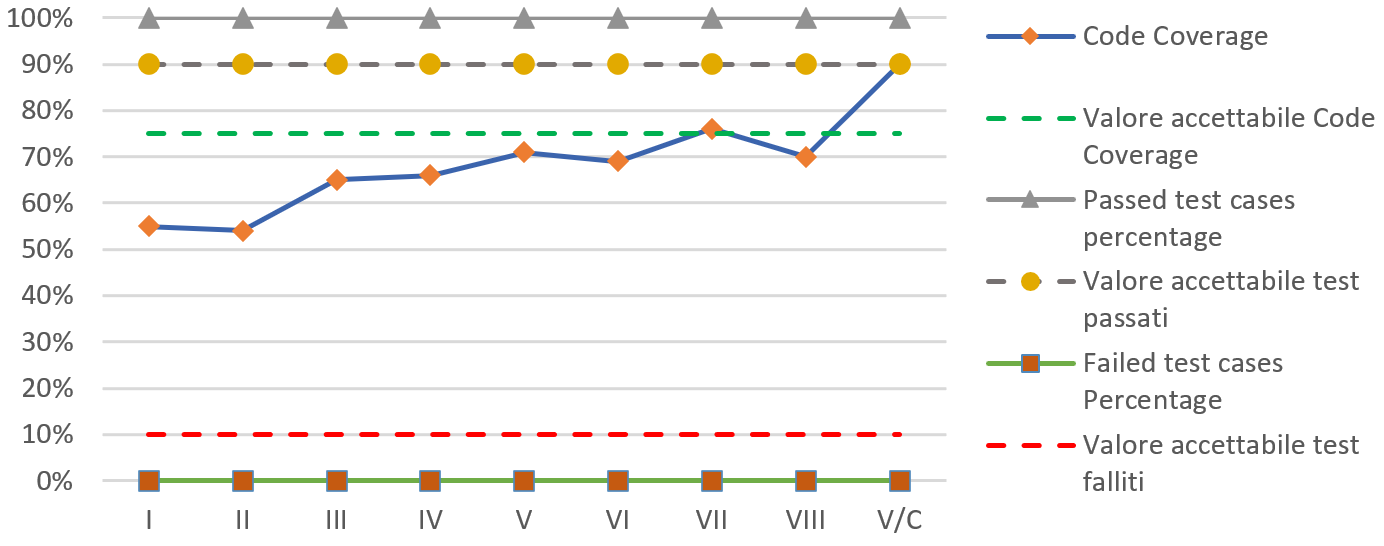
\includegraphics[width=17cm]{Images/codeCov}
	\caption{Copertura del codice e percentuale di test superati e falliti per incremento.}
\end{figure}

\subsubsection{Densità di failure}
\begin{figure}[h]
	\centering
	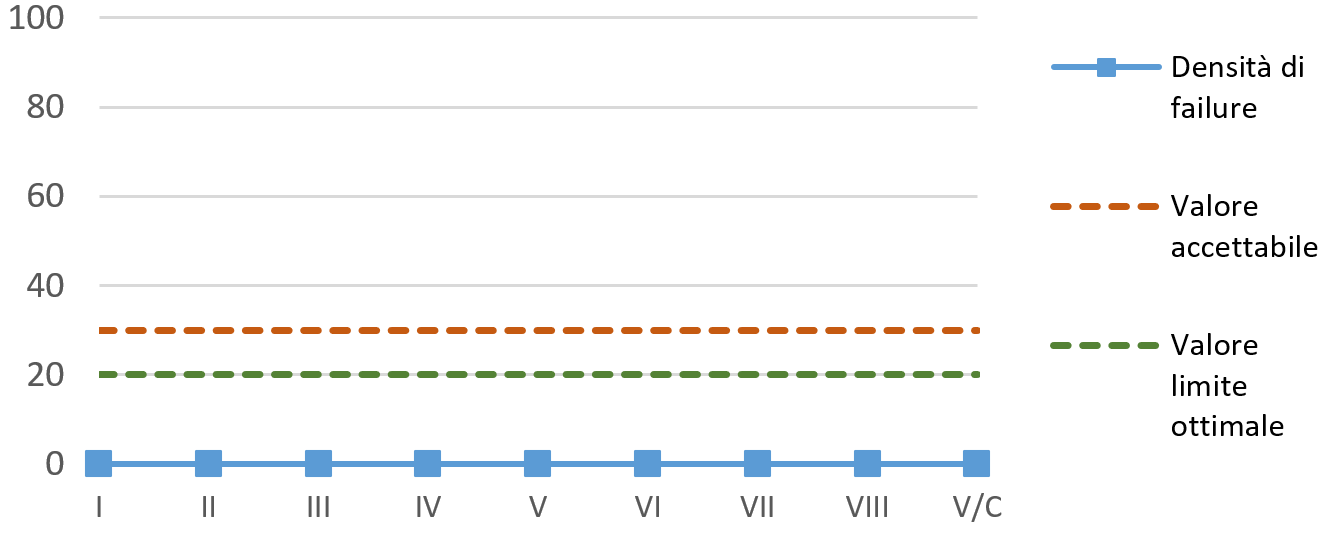
\includegraphics[width=15cm]{Images/densFailure}
	\caption{Percentuale di test falliti sui totali per incremento.}
\end{figure}

